\chapter{Introducción}

\section{Conceptualización}

La escuela (salesiana) al alcance de los más necesitados en Irapuato es un bachillerato tecnológico que se pretende crear en dicha ciudad con el doble objetivo de brindar una capacitación técnico-académica de calidad a nivel bachillerato y de ofrecer una educación integral en valores según el sistema educativo de Don Bosco a los jóvenes más necesitados.

\subsection{Origen de la Idea}

La idea original nace en el seno de la Comunidad Salesiana <<María Reina de Irapuato>> la cual ante la problemática social enfrentada por las familias en esta ciudad, tales como  la ruptura familiar, las adicciones y el analfabetismo, propone la realización de este proyecto, al validar que, ante la interrogante <<¿Qué estamos haciendo por los pobres?>>, no se tiene una respuesta plenamente satisfactoria puesto que las estadísticas locales, la entidad presenta elevados índices en las variables antes mencionadas.\citep{Morales09}

Ante esta situación, el Pbro. Edmundo Morales Romero, S.D.B, sacerdote salesiano miembro de dicha comunidad, destaca la existencia de numerosas razones por las cuales es urgente emprender una labor educativa a fondo y de largo alcance que impacte en el desarrollo local dentro de su ámbito de influencia en primera instancia y en un futuro próximo sea susceptible de reproducción en las demás entidades del país.

Este modelo pretende cubrir desde un sector cuyo nivel económico le permita pagar una colegiatura hasta aquel para el que es del todo imposible hacerlo por si mismo.

Al bachillerato podrán ingresar todos aquellos que hayan acreditado la secundaria. Las clases las tomarán todos juntos evitando todo tipo de discriminación y eliminando una barrera de la historia reciente en nuestro país: la diferencia entre los que van a escuela de paga y a escuela pública.

El perfil de egreso es el de bachillerato de alta calidad con una carrera técnica adecuada a las características de la región.

\subsection{Notas Distintivas}
\label{sub:intro:NotasDistintivas}

La escuela tiene como rasgos distintivos aquellas características del modelo educativo de Don Bosco, y que pueden resumirse en 5:

\begin{description}
	\item[Sistema preventivo] En contraposición al sistema represivo, se trata de ganar a los estudiantes con amabilidad para orientarlos al bien. A los 9 años, Don Bosco tuvo un sueño en el que Jesús le decía: \emph{no con golpes, sino con la mansedumbre y la caridad deberás ganarte a estos tus amigos}\footnote{San Juan Bosco, Memorias del Oratorio en \citep{Canals95}}.

	\item[Acompañamiento] Los jóvenes nunca están solos, incluso en los ratos de descanso y esparcimiento siempre hay alguien que los acompaña y convive con ellos.
	
	\item[Formación en valores] El sistema preventivo, en palabras de Don Bosco, sólo funciona si se basa en el Evangelio, en una sólida vida interior apoyada en los sacramentos. De aquí se desprende todo lo demás\footnote{San Juan Bosco, en \emph{El Sistema Preventivo en la Educación de la Juventud} (1877) nota 1, \citep{Canals95}. El texto de la nota puede verse íntegro en el Apéndice \ref{ap:preventivo}, página \pageref{ap:preventivo}}.

	\item[Quitar barreras de discriminación] En un mismo salón de clase convivirán jóvenes de todos los estratos sociales, a los cuales se les brindará el mismo trato promoviendo la amistad entre ellos.

	\item[Formación para el trabajo] Mediante las carreras técnicas y los talleres se procurará que los jóvenes tengan la posibilidad de conseguir un empleo ya sea de tiempo parcial para seguir estudiando o si las circunstancias se imponen, de tiempo completo.
\end{description}

\section{Objetivos}

\subsection{Objetivo General}
\label{sub:ObjetivoGeneral}

El presente trabajo tiene el siguiente objetivo general:

\begin{quotation}
	Verificar la viabilidad financiera de la Escuela Salesiana mediante el análisis del punto de equilibrio, indicadores financieros y evaluación financiera para así decidir si se realiza el proyecto como está conceptualizado o se buscan alternativas.
%	Verificar la viabilidad financiera de la Escuela Salesiana mediante el análisis de su corrida financiera para así decidir si se realiza el proyecto como está conceptualizado o se buscan alternativas.
\end{quotation}

%El objetivo general del presente trabajo es verificar la viabilidad financiera de la Escuela Salesiana.

%La viabilidad financiera se entiende en el sentido de que el bachillerato puede ser un negocio redituable.

\subsection{Objetivos Específicos}

El trabajo precisa los siguientes objetivos específicos para garantizar el cumplimiento del objetivo general:

\begin{itemize}
	\item Determinar el monto total de la inversión inicial, mediante el análisis de las necesidades de liquidez e infraestructura, para así establecer la situación patrimonial inicial de la Escuela.
	\item Determinar las fuentes para el financiamiento inicial mediante la diferenciación entre el financiamiento patrocinado y la adquisición de deuda para precisar las obligaciones de largo plazo (pasivos) a cubrir.
	\item Verificar la viabilidad financiera cuidando que siempre se rebase el punto de equilibrio, igualmente, garantizar que las razones financieras indiquen un resultado favorable para así asegurar que la Escuela puede \emph{valerse por sí misma}.
	\item Determinar la cobertura máxima de becas expresada en porcentaje sobre el total de los ingresos mediante el ajuste entre los egresos y los ingresos para así medir a cuántos estudiantes puede beneficiar la escuela si considera como fuentes de ingreso únicamente las de la inversión inicial y las colegiaturas.
	\item Identificar el punto de equilibrio considerando exclusivamente la inversión inicial y las aportaciones de los estudiantes (colegiaturas) para así evaluar la capacidad de la escuela para ofrecer becas.
	\item Verificar si el proyecto, así concebido, es además, rentable desde el punto de vista lucrativo, a través del análisis de las variables de evaluación financiera,\footnote{\label{note:VariablesEvaluacionFinanciera}Período de Recuperación Simple y Descontado, Retorno sobre la Inversión, Valor Presente Neto, Tasa Interna de Rendimiento e Índice de Rentabilidad} lo cual ayudará a la comunidad salesiana de Irapuato a definir su estrategia para la obtención del financiamiento que requiere.\footnote{La estrategia para la obtención del financiamiento externo queda excluida del presente trabajo.}
\end{itemize}

\section{Alcances, Limitaciones y Supuestos del Proyecto}

\subsection{Alcances}

%El presente trabajo abarca únicamente el plan financiero y los aspectos que directa o indirectamente impactan en él.

%¿qué se va a hacer en el trabajo?

Para asegurar el logro de los objetivos antes descritos, el presente trabajo presenta el plan financiero a cinco años de la Escuela Salesiana que se pretende formar.

%¿cómo se va a realizar?

Dicho plan contempla la elaboración de una corrida financiera, así como el análisis del punto de equilibrio, las razones financieras y una evaluación financiera del proyecto.

La corrida financiera se basa en la preparación de presupuestos de ingresos y egresos, los cuales, a su vez, se apoyan respectivamente en un análisis preliminar del mercado y en la especificación de las operaciones y necesidades de inversión a realizar. 

El análisis del punto de equilibrio, así como el de las razones financieras y la evaluación financiera provienen de la corrida financiera, principalmente de los estados financieros proforma: estado de resultados, balance general y flujo neto de efectivo.

%¿qué se espera obtener?

Al final se espera obtener la información que permita determinar si el proyecto es viable de acuerdo con los objetivos general y específicos mencionados.

%¿cuáles son los criterios de éxito?

Las variables a considerar para determinar el éxito del proyecto, son las razones financieras y las utilidades en el estado de resultados y flujo neto de efectivo.

%De los cinco años que se están analizando, al menos los tres últimos deben arrojar utilidades (estado de resultados, rebasar el punto de equilibrio), y tener valores aceptables en las razones financieras; en cuanto al flujo neto de efectivo, al menos el último año debe ser positivo, lo cual significa que la escuela recupero completamente su inversión.

%¿cómo se van a interpretar los resultados?

Si el proyecto rebasa el punto de equilibrio (i.e. el estado de resultados tiene saldo positivo), las razones financieras son favorables y al final el flujo neto de efectivo es positivo; entonces el proyecto es viable. Si falla alguno de estos tres criterios, entonces se debe replantear el modelo.

En cuanto a la evaluación financiera,\footnote{Ver nota \ref{note:VariablesEvaluacionFinanciera}, página \pageref{note:VariablesEvaluacionFinanciera}} ésta cumple otro propósito, mientras mejores sean los resultados arrojados por estas variables, más fácil será obtener el financiamiento y apoyo requerido; si los resultados no son favorables, deberá realizarse un mayor esfuerzo en la elaboración y ejecución de la estrategia de la búsqueda de apoyo y financiamiento externos.

\subsection{Limitaciones}

%%%%%%%%%%%%%%%%%%%%%%%%%%%%%%%%%%%%%%%%%
% se refiere a las limitaciones del trabajo de investigacion/plan financiero, no a las limitaciones del modelo de la escuela salesiana
%%%%%%%%%%%%%%%%%%%%%%%%%%%%%%%%%%%%%%%%%

%- ¿que cosas relacionadas con el objetivo general quedan fuera del trabajo?

%	-- justificacion del objetivo?
%	-- alternativas?
%	-- "como esta conceptualizado" ==> fundamentar ??

%- ¿que cosas relacionadas con los objetivos especificos quedan fuera del trabajo?

%	-- justificacion de la infraestructura?
%	++ viabilidad y origen preciso del financiamiento patrocinado
%	-- institucion crediticia exacta para solicitar el prestamo?
%	-- si el proyecto cumple o no con las condiciones para solicitar el prestamo?
%	-- precicion del termino "favorable" en las razones financieras?
%	-- por que unicamente se consideran las colegiaturas como fuente de ingresos?
%	-- justificacion de las variables de evaluacion financiera?
%	++ la estrategia de la comunidad salesiana para conseguir el financiamiento requerido
%	-- justificacion de la TREMA ?

%- ¿qué qué cosas relacionadas con el alcance quedan fuera del trabajo?

%	-- fuentes para definir la estructura del plan financiero?
%	-- definicion de corrida financiera?
%	-- estudio de mercado "a fondo"?
%	-- justificacion de los criterios de exito?
%	-- la estrategia para conseguir el financiamiento externo

El actual trabajo presenta como limitantes, las que se enumeran a continuación:

\begin{itemize}
	\item Se excluye del presente trabajo la investigación que determine si es viable y bajo qué condiciones las empresas y otros actores sociales patrocinarían el proyecto.
	\item Igualmente queda excluida la estrategia que utilizará la comunidad salesiana para conseguir dichos patrocinios.
	\item No se contemplan fuentes de ingresos adicionales a las especificadas en la inversión inicial y las aportaciones directas de los estudiantes. Aunque se mencionan algunas, únicamente es con propósito ilustrativo, más no se consideran para determinar la viabilidad financiera de la escuela.
	\item No se incluye el estudio de mercado que determine el número máximo de personas que se inscribirían a la escuela considerando diferentes montos de colegiatura. % no se si mencionar esta
	\item El horizonte de evaluación es a cinco años a partir del inicio del proyecto. % metodologia
	\item Todos los datos y cálculos se basan en la información recopilada hasta el año 2010. % metodologia
\end{itemize}

%%%% esto es viejo, ver si se mueve a la prefactibilidad o a otra area %%%%

%El modelo de financiamiento es múltiple: aportaciones directas (colegiaturas), fondos privados, apoyos públicos, servicios a empresas, entre otros.

%Se cobrará una aportación monetaria en función de las capacidades de cada alumno. El objetivo es financiar a los jóvenes de escasos recursos mediante las aportaciones de los estudiantes con posibilidades económicas. Se buscarán fondos privados para becas e infraestructura en diversas modalidades: apadrinar alumnos con buenas calificaciones, apoyos para proyectos específicos: laboratorios, talleres, etc.; apoyos en especie.

%Se intentará obtener apoyos públicos en función de la labor social que se realiza a través de programas como Oportunidades, Practica-Trabaja, Lazos, Bécalos, Prepa Sí, etc.

%Entre otras actividades para obtener ingresos se contemplan: prácticas profesionales patrocinadas por empresas (venta de servicios de acuerdo a carrera técnica y necesidades de las empresas locales); programas de reciclaje; rifas, noches coloniales y eventos de sano entretenimiento, etc.

%Como actividades formativas y simultáneamente ahorradoras se consideran las siguientes: aportaciones en especie de los miembros de la comunidad, jornadas de limpieza, pintura y reparación; servicio en la cooperativa (tienda de la escuela), etc.

\subsection{Supuestos}
\label{sub:Supuestos}

%supuestos: Objeto y materia que no se expresa en la proposición, pero es aquello de que depende, o en que consiste o se funda, la verdad de ella. (recordar en el marco teórico-metodológico)
%- cuáles supuestos tiene el proyecto que lo determinan y que provocaron problemas en la exposición pasada
%- cuáles supuestos tiene el proyecto que lo determinan y aunque no causaron problemas, sí podrían provocarlos en la próxima exposición
%- por qué se dieron estos supuestos

Todo proyecto se apoya en supuestos con la finalidad de cubrir aquellas lagunas que son consecuencia natural de la incertidumbre al momento de realizar la planeación; éstos deberán se confirmados o rechazados durante la puesta en marcha del plan y en dado caso de verificarse falsos, reelaborar el proyecto.

Los supuestos en los que se basa este proyecto son los siguientes:

\begin{itemize}
%	\item Se considera que la aprobación por parte de la inspectoría es un hecho aunque podría demorarse, en caso de hacerlo hay que realizar ajustes en el plan, dichos ajustes no se contemplan en el presente trabajo.
	\item Se da por sentado que se contará con los patrocinios y el préstamo necesarios para arrancar el proyecto. La confirmación de este supuesto deberá realizarse a través de sondeos entre posibles patrocinadores y entidades crediticias una vez obtenida la aprobación por parte de los superiores de la congregación salesiana (la inspectoría). Los mencionados sondeos no se incluyen en el presente trabajo.
	\item El modelo de negocio a evaluar es el que generalmente tienen los colegios particulares, con la salvedad de que la inversión inicial incluye un patrocinio y que las utilidades se reinvierten en la misma escuela. Se eligió este modelo con el fin de conocer la capacidad de la escuela de sostenerse y ofrecer becas por sí misma. La exploración de otros modelos no se incluye en este trabajo.
\end{itemize}

\section{Prefactibilidad}

\subsection{Aspectos Previos - Situación Actual}
\label{sub:Intro:AspectosPrevios}

El estado de Guanajuato enfrenta diversos problemas sociales derivados de una oferta educativa insuficiente:
%(Cf. \citep{Morales09}):

\begin{description}
	\item[Educación] Guanajuato es una de las entidades con mayor índice de analfabetismo a nivel nacional.\footnote{Según el Conteo de Población y Vivienda 2005 \citep{Inegi2005}, Guanajuato ocupa el quinto \emph{último} lugar en escolaridad con 7.1 años en promedio contra 8.1 nacional.} Concentrándose la mayor cantidad de analfabetas \emph{en las zonas urbanas}.\footnote{\citep{Morales09}}
	\item[Desempleo] El desempleo asciende al 6\% de la población económicamente activa.\footnote{\citep{Inegi2010Enoe}}
	\item[Niños de la calle] Guanajuato es de los principales estados receptores de niños de la calle.\footnote{\citep{Morales09}}
	\item[Ruptura familiar]
	Guanajuato pasó del lugar 22º al 19º en divorcios entre los años 2005 y 2009\footnote{Comparar \citep{Inegi2005pGto} con \citep{Inegi2009pGto}} con el consecuente semi abandono de los niños.\footnote{\citep{Morales09}}
	%Guanajuato está en el 4º lugar de divorcios, ha aumentado un 400\% en estos últimos años, con el consiguiente semi abandono de los niños.
	\item[Delincuencia] Al igual que el resto del país, la entidad padece un incremento en los índices delictivos y de violencia.\footnote{\citep{CIDE2010}}
\end{description}

\subsection{En Caso de no Llevarse a Cabo}

En caso de no llevarse a cabo el proyecto, estos índices aumentarían con grave daño a la sociedad local.

Por otra parte, el gran desarrollo industrial del Estado se vería afectado y la comunidad no podría aprovechar este beneficio, al no contar con la preparación técnica necesaria, las empresas contratarían personal foráneo para cubrir sus necesidades de talento humano.

\subsection{Ubicación}

Se cuenta con un inmueble ubicado en la zona centro de Irapuato, abarca toda la manzana delimitada por las calles: Díaz Ordaz, Francisco Sarabia, Río Grijalba y Lázaro Cárdenas, se puede observar una foto satelital en la figura \ref{fig:ubicacion}.

\begin{figure}
	\centering
	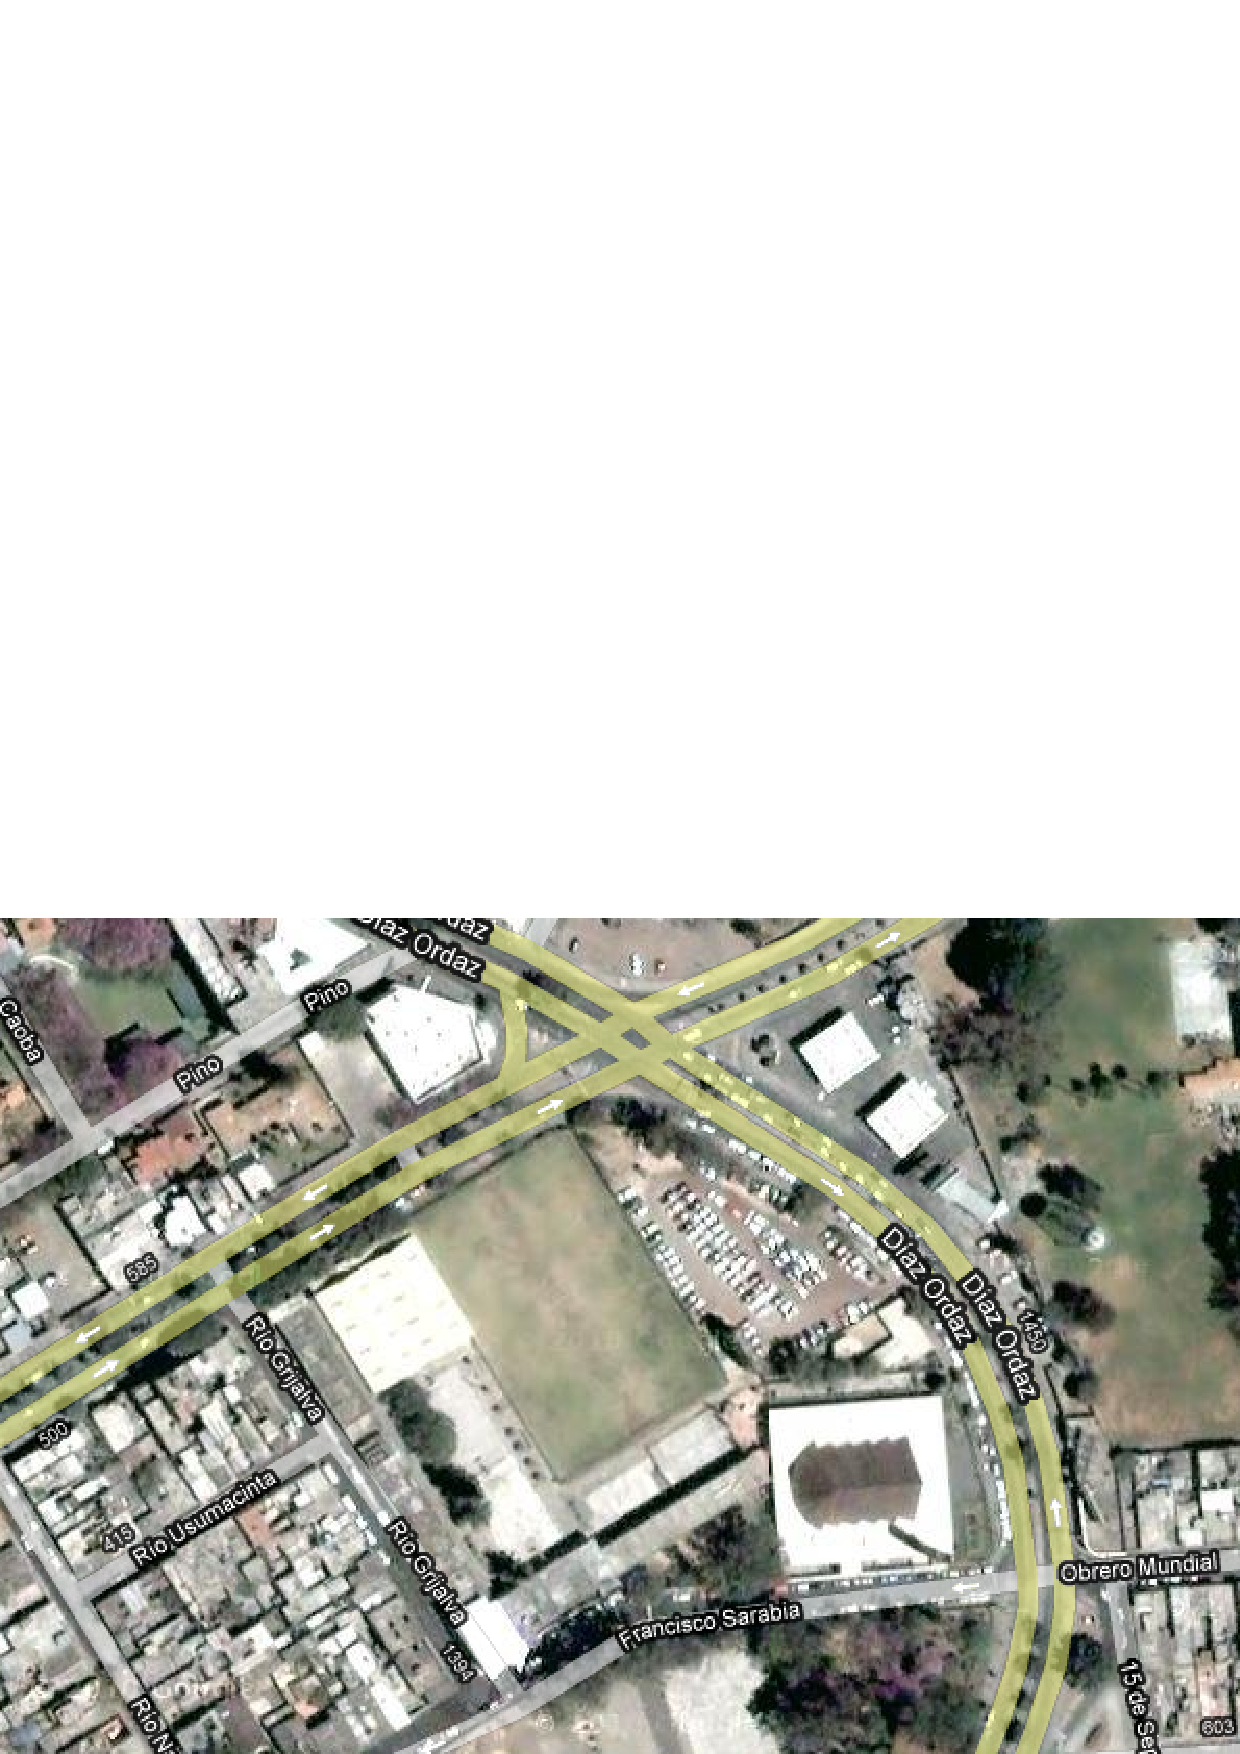
\includegraphics[scale=0.5]{images/localizacion}
	\caption[Fotografía satelital y ubicación del inmueble.]{Fotografía satelital y ubicación del inmueble.\newline Fuente: \citep{GoogleMaps2010}}
	\label{fig:ubicacion}
\end{figure}

\subsection{Evaluación Financiera Previa}

\subsubsection{Infraestructura Actual}

Se cuenta con un inmueble adaptado como escuela, al cual, actualmente no se le da este uso; aunque requerirá modificaciones menores ya tiene la capacidad de atender a más de 1,000 alumnos en 40 aulas.

La superficie del inmueble es de 14,452 $m^2$ con un valor aproximado de \$ 3.4 millones de pesos; los edificios están valuados en \$ 2.4 millones de pesos aproximadamente.

%\footnote{Valor estimado con base en el precio por metro cuadrado promedio en Irapuato \citep{AM2010}}.

\subsubsection{Beneficio Social}
\label{sub:sub:Beneficio:Social}

La intención es cubrir al menos un 40\% del alumnado con alguna beca. Por comparación, un bachillerato salesiano en Jalisco orientado como \emph{escuela privada} otorga un 20\% en becas.

Considerando la capacidad actual del inmueble el beneficio social que se espera obtener es el equivalente a 400 jóvenes atendidos de forma completamente gratuita. Sin embargo, la intención es distribuir las becas utilizando porcentajes, por lo que la cobertura real deseada es que más de la mitad de la población estudiantil se vea beneficiada con algún tipo de beca.

Por otra parte, la educación en valores basada en el sistema preventivo de Don Bosco beneficiará todos los estudiantes y a sus familias.

\subsubsection{Capacidad actual}

Se pretende dividir a los alumnos en grupos de 30 estudiantes como máximo. De acuerdo con el sistema salesiano, esto da como resultado un total de 37 personas atendiendo directamente a los estudiantes.

La colegiatura estándar en la región es de \$3000.00 mensuales, lo cual, aplicado a 600 estudiantes durante un año da como resultado un monto de \$21,600,000.00. A esta cantidad habrá que añadir lo que se obtenga mediante donativos y patrocinios.

\subsubsection{Patrocinios}
\label{sub:Patrocinios}

Las experiencias similares en Saltillo y San Luis Potosí\footnote{Entrevista con el Pbro. Edmundo Morales Romero, S.D.B., 11 de septiembre de 2011} muestran que esta clase de proyectos son bien recibidos por los industriales locales; en efecto, en ambas entidades, los grupos industriales realizaron aportaciones en efectivo y en especie a tal grado que incluso donaron los terrenos a cambio de adaptar los planes de estudio a sus necesidades.

Irapuato se ubica en el centro del eje industrial de Guanajuato, el cual incorpora a las ciudades de León, Silao, Irapuato y Salamanca. En toda esta zona existen diversos parques industriales e industrias de todo tipo. Próximamente se abrirá una planta de fabricación de componentes espaciales, la cual estará necesitada de mano de obra calificada. Todas estas industrias son candidatos a ser patrocinadores del proyecto por así convenir a sus intereses.
